%%%%%%%%%%%%%%%%%%%%%%%%%%%%%%%%%%%%%%%%%%%%%%
\logvartrue
\chapter{Background}
%%%%%%%%%%%%%%%%%%%%%%%%%%%%%%%%%%%%%%%%%%%%%%

Bacteria are often cited as examples of one of the Earth's most primitive living forms. Unfortunately, they are still associated almost exclusively to infection diseases, but the reality is rather different. Indeed, only a very small fraction of bacteria is able to cause infections in contrast to a highly diversified and beneficial bacterial world. Most of them not only reciprocally support each other but their immensely varied and efficient metabolism also defines and sustains balanced environments (the biosphere). Solidarity among bacterial cells is one of their most important characteristic. Even infection-causing bacteria are able to benefit from this solidarity, making them more resilient and ``inventive'' than isolated species \cite{mathieu1995powerful}. In the last 20 years, the development of genomic tools has revolutionized microbial ecological studies and strongly expanded our view on this previously under appreciated microbial world. It is encouraging to see that evolution and ecology are now emerging as regular subjects within microbiology. The next decade should be one of gradually changing and enlarging perspective regarding the place of microbiology in the biological sciences. There are now comforting signs that we are moving towards a deeper and more realistic appreciation of the roles played by bacteria on our planet.

\section{The Bacterial world}
Microorganisms are essentially everywhere in nature and they have been integral to the history and function of life on Earth. However, until very recently, their importance has been appreciated by only a few specialists. Indeed, bacteria are still most often considered from an anthropocentric point of view, focusing our attention only on the relatively few pathological species or their potential to provide us with useful products and services. This is a very constrained perspective if we think that bacteria have been the sole form of life on Earth for some two billion years, playing central roles in climatic, geological, geochemical, and biological evolution \cite{cavalier2006cell}.\\
The bacterial world contains a highly heterogeneous group of organisms sharing only one common characteristic, their small size. The patterns of bacteria distribution are influenced by environmental factors such as temperature, pH, salinity, pressure, the presence of nutrients and the sources of carbon and energy \citep{gerhard1986bacterial}. These factors are able to shape Earth's bacterial community distribution with respect to both space and time, influencing the selective proliferation of a set of bacteria in a distinct environment, based on their metabolic characteristics. Bacteria can use many different types of metabolic strategies and bacterial species can often be differentiated from each other based on their metabolic characteristics. The specific metabolic properties of a microbe are one of the major factors in determining that microbe’s ecological niche, and they can be used to classify bacteria in different metabolic groups (Figure~\ref{fig:bacmet}). Thanks to their high variability, bacteria have been, and still are, able to colonize almost every habitat in nature.\\
\begin{figure}[!tb]
	\centering
	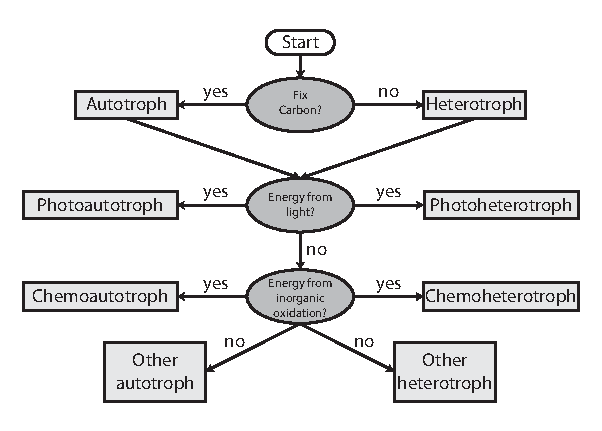
\includegraphics[width=0.7\textwidth]{./figures/Introduction/bacterial_metabolism_bw}
  	\caption{General flowchart used for metabolic classification of bacteria. \label{fig:bacmet}}
\end{figure}
Giving their ability to thrive in a vast set of different environments, bacteria play pivotal roles in several biogeochemical cycles and are responsible for the cycling of organic compounds. They have been found in all kind of environments ranging from the human gut \cite{walter2011human}, to the rhizosphere \cite{philippot2013going}, to conventionally inhospitable habitats such as acid mine run-off \cite{simmons2008population} and geothermal hot springs 	\cite{sharp2014humboldt}. Studies based on cultured microbes have revealed that they are critical components of these environments providing them with essential services \cite{van2008unseen, arrigo2004marine}. For example, the Earth's cycles of hydrogen, carbon, nitrogen, oxygen and sulphur are driven largely by microbial catalysed redox reactions. These reactions require multimeric protein complexes evolved exclusively in microorganism such as bacteria \cite{falkowski2008microbial}. However, a large part of these processes is still unknown making the study of bacterial functions indispensable for the complete comprehension of the dynamics able to modify our planet.\\
Biologists have long appreciated the roles that microbes play in the two distinct disciplines of pathogenesis and ecosystem cycling; although, in these years, the importance of microbes-host association is rapidly growing. Currently, microbes associated with a macroscopic host have their own definition in the word ``microbiota'' coined for the first time by Joshua Lederberg in 2001 \citep{lederberg2001scientist}. The role of microbiota is occupying a very important position in the host evolution \cite{ley2008evolution}. Indeed, the set of bacteria linked with a macroscopic organism can interact with its host to influence physiology and contribute to health, growth, or fitness \citep{dimkpa2009plant, hooper2012interactions}. For example, studies of model rhizosphere microbiota have taught us that they can impact plant growth \citep{kennedy2007competitive}, stress response \cite{redman2002thermotolerance, yang2009rhizosphere}, and pathogenic defense \cite{cook1995molecular}. In this perspective, for understanding completely a macroscopic organism’s physiology is becoming mandatory the investigation of its microbiota.\\
This great microbial diversity found in various environments (including hosts associated ones) can be measured by a set of indices such as phylogenetic diversity, species diversity, genotype diversity, and gene diversity. Above the species level, microbial diversity has been commonly quantified based on evolutionary distances among observed taxonomic groups from a specific environment. Below this level, microbial diversity has been typically described using population genetic parameters such as gene diversity and genotype diversity. However, despite the fact that species is the fundamental unit of biological classification, what constitute a species remain controversial. In addition, until very recently, most of what we know about microbial diversity and microbial functions were derived from cultured microorganisms. While such studies are essential, the advent of genomic has revolutionized our comprehension of the bacterial world showing that much of what we thought we knew about this microscopic world were in fact highly biased.\\

\subsection{The species concept}
Attempting to bring order in the astounding variety of organisms with which we share the planet have been an endless human effort. One of the first classification system was developed by Carl Linnaeus in the mid-18th century in his works \textit{Systema Naturae} and \textit{Species plantarum} \cite{linnaeus1800species, bhl10277}. Linnaeus established the existence of three kingdoms: the animal kingdom (\textit{Regnum animale}), the plant kingdom (\textit{Regnum vegetabile}) and the mineral kingdom (\textit{Regnum lapideum}), laying the foundation for a hierarchical classification of the natural world. In his works Linnaeus did not classify microbes but, since the mid-19th century, his binomial nomenclature has been used by microbiologist to designate microbial species. However, what constitute a species was, and remains, controversial especially with the advent of the ``genomic era'' and the explosion of data that it has brought with it \cite{doolittle2006genomics}.\\
\begin{figure}[!tb]
	\centering
	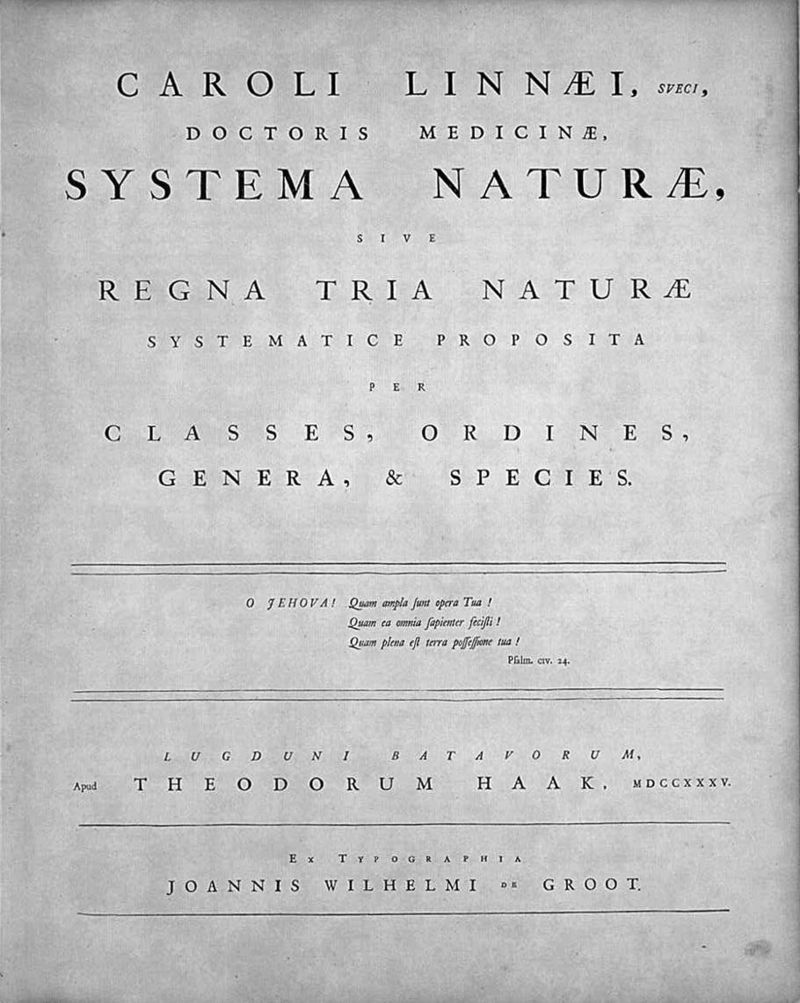
\includegraphics[width=0.3\textwidth]{./figures/Introduction/systema_naturae}
	\caption{The title page of Systema Naturae, Leiden (1735)}
\end{figure}
Prokaryotic classification is the youngest and most dynamic between all classifications of living organisms. This might be due to the fact that prokaryotes were not even know to exist until a few centuries ago. Moreover, developing a prokaryotic classification system based on macro-morphological traits, like sexual reproduction or some physical characteristics, is impossible because of their relative simplicity \cite{cowan1965principles}. The absence of useful fossil records, together with the difficulties in identifying possible diagnostic elements from these organisms have concur to the instability of the prokaryote classification system. Indeed, species demarcation in prokaryotes is not defined by a theory-based concept and tends to be more arbitrary, anthropocentric or rooted in practical necessity (e.g. bacteria species like \textit{Neisseria meningitis} or \textit{Bacillus anthracis} have been historically defined based on the disease they cause regardless of other types of considerations).\\
Until the end of the 18th century, no prokaryotic classification was attempted. Ottu M\"{u}ller, a Danish naturalist, was the first to create a systemic arrangement of microorganisms defining two form genera called \textit{Vibrio} and \textit{Monas}; which differentiated the round and elongated type of bacterial cells \cite{logan2009bacterial}. One of the most important step in the classification of microorganisms was the ability to isolate them in pure cultures. Therefore, in 1881, Robert Koch published the first technique of cultivation on solid media; paving the way for what he called ``the golden age of the medical microbiology''. Following this discovery, researchers were able to retrieve direct informations on a microorganism by cultivating it in pure culture; thus, the amount of bacteria described from the end of the 19th century to the first two decades of the 20th century was impressive. In 1970  a modern identification index for bacteria was first provided with the publication of the ``Bergey's Manual of Determinative Bacteriology''. In the second half of the 20th century the increasing knowledge of the properties DNA, in conjunction with the development of molecular biological techniques pushing the idea that bacteria might be classified using their genomes. Finally, in 1970, the catalogation of the ribosomal RNA (rRNA) and the development of the DNA-DNA hybridization technique permitted to achieve a great breakthrough in the history of bacterial classification \cite{stackebrandt198516, de1975improvements}.\\
Currently, microbial species are defined using the so-called ``polyphasic approach'', that is grounded on clear rules for both genotypic and phenotypic attributes \cite{vandamme1996polyphasic}. Nowadays, more than 7000 different microbial species have been classified using this approach, but, as actually practised, it faces serious problems. Indeed, the primary criterion for discriminating between different species is a cut-off level for pairwise genomic DNA-DNA hybridization levels; however, this cut-off level has never been based on any particular theoretical assumption \cite{de2005ernst, hey2006failure}. Furthermore, pairwise comparison of microbial strains can be asymmetric (different values can be obtained with the same pair of strains simply exchanging the one used as probe with the one used an target) and intransitive (hybridization levels > 70\% between strains A - B, and A - C may be not necessary the same between B - C). Moreover, a large number of surveys of microbial diversity have equalled species with ``operational taxonomic units'' (OTUs) based on 16S rRNA sequence \cite{ley2006microbial}. However, although 16S rRNA can be used for comparing and classifyning known species, it may have insufficent genetic resolution for the de-novo binning of newly isolated microbes into species. For these reason, newer genomic methods have been developed recently consisting in the identification of discrete sequence clusters based on multiple core genes \cite{fraser2007recombination, gevers2005re}. But all these technical issues are not able to address a primary conceptual question: what is a microbial species?\\
From the beginning of the 20th century the species concept has been redefined multiple times. The first species concept universally accepted was the one developed by Ernst Mayr and then called ``the biological species concept'' (BSC) \cite{mayr1942systematics}. This concept defines species as groups of ``potentially interbreeding natural population which are reproductively isolated from other such groups''. Unfortunately, this definition is not applicable to asexual organisms lacking a meiotic life cycle, as bacteria. In the modern era, other two distinct species concepts have been developed, and both of them are currently accepted by biologist and philosophers. The first one is the ``phenetic species concept'' (PhSC); it is based on ``statistically co-varying characteristics which are not necessarily universal among the members of the taxa'' \cite{claridge1997species, sokal1970biological}. The second one is the ``evolutionary species concept'' (ESC) that defines a species as ``an entity composed of organisms which maintains its identity from other such entities through time and over space, and which has its own independent evolutionary fate and historical tendencies'' \cite{claridge1997species}. However, none of these concepts was specifically developed for the definition of the microbial species; for this reason, several other attempts to fill this gap have been suggested. Below is reported a collection of the most representatives definition of microbial species in order to highlight the lack of consensus:
\begin{itemize}
\item ``A species could be described as a monophyletic and genomically coherent cluster of individual organisms that show a high degree of overall similarity in many independent characteristics, and is diagnosable by a discriminative phenotypic property'' \cite{rossello2001species}.
\item ``Species are considered to be an irreducible cluster of organisms diagnosably different from other such clusters and within which there is a parental pattern of ancestry and descent'' \cite{staley2006bacterial}.
\item ``A species is a group of individuals where the observed lateral gene transfer within the group is much greater than the transfer between groups'' \cite{dykhuizen2005species}.
\end{itemize}
One of the newest concept developed is the so-called method free unitary concept, which defines microbial species as ``metapopulation lineages'' \cite{de2005ernst}. Here, a metapopulation is defined as a set of connected subpopulations and a lineage can be thought of as a metapopulation that extends through time and evolves separately from other lineages (Figure~\ref{fig:metapop}). Following this criterion a species does not need to be ``phenotypically distinguible, or diagnosable, or monophiletic, or reproductively isolated, or ecologically divergent, to be species''. The only criterion for a species according to this concept is their evolutionary fate, and no methodological criterion is required for assigning species designations. Although this new conception of microbial species still has not been fully accepted, it continues to have
important consequences. For example its more complete acceptance may provide a solution to the species concept problem, bringing the species concept into line with claims about the general theoretical significance of the species category.\\
\begin{figure}[!tb]
	\centering
	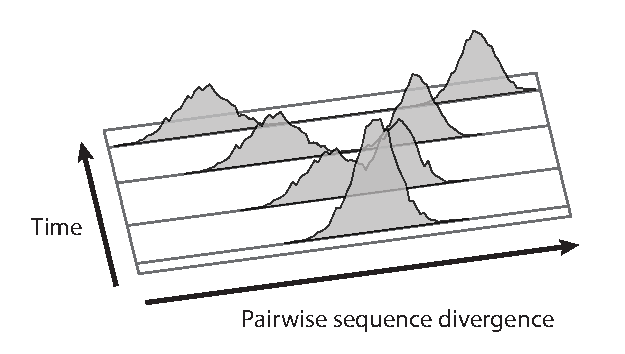
\includegraphics[width=0.7\textwidth]{./figures/Introduction/metapopulation}
  	\caption{Frequencies of binned levels of pairwaise genetic divergence. This schematic representation shows the generation of two distinct populations over time. \label{fig:metapop}}
\end{figure}
Defining the  concept of species for prokaryotes remains a problematic task, despite microbiologists and philosophers have undertaken several efforts to find a correct and shared working scheme. The emergence of new definitions for microbial species is gradually changing the whole concept of prokaryotic evolution in the attempt to find methods and thresholds indipendent criteria. This is giving new life to the study of bacterial genomes as a possible and more comprehensive way for measuring the distance between two different ``metapopulation lineages''.\\

\subsection{Microbial diversity}
Studying natural species in their environment has always been one of the crucial task in Biology and Ecology. For centuries, biologists have studied pattern of plant and animal diversity in different ecological niches; but, until recently, these kind of analyses were impossible for microorganisms even if they were, and still are, one of the most diverse and abundant group of organisms on Earth \cite{curtis2005exploring}. New genetic techniques have revealed extensive microbial diversity that was not possible to to detect with culture-dependent methods. Even though the application of these new techniques, the scientific understanding of the microbial distribution patterns is still particularly weak. The definition of new diversity estimators specifically designed for microbial life is needed to fully comprehend the role of microorganisms on the planet.\\
In order to inspect the complexity of a natural community the first thing that we ask ourselves is: how many different species there are in that community? In other words what we want to know is the ``species diversity'' of the community that we are studying. Species diversity is an abstract measure composed by two components: ``species richness'' and ``species evenness''. The first component is a measure of the number of different species found; whereas, the latter quantifies how equal the abundances of these species are \cite{hill1973diversity}. In general, species diversity reflects the variety of organisms present in a particular environment; although, speaking about living organisms in an environment requires some considerations. First of all, the community of living organisms able to interact with non-living components of their environment is called an ``ecosystem''. In addition, a single ecosystem can be considered as a composition of multiple small habitats that, in turn, may be considered as ecosystems. Giving this great variability how can we refer to the diversity of a single ecological niche or to the whole diversity of an ecosystem?\\
The species diversity of a particular ecosystem is called $\gamma$-diversity and is the sum of two others sub-diversities: the $\alpha$-diversity and the $\beta$-diversity \cite{whittaker1960vegetation}. The term $\alpha$-diversity refers to the mean species diversity in a locale scale like an habitat or a particular site; whereas, the term $\beta$-diversity refers to the differentiation among those habitats or sites (Figure~\ref{fig:diversities}). 
\begin{figure}[!tb]
	\centering
	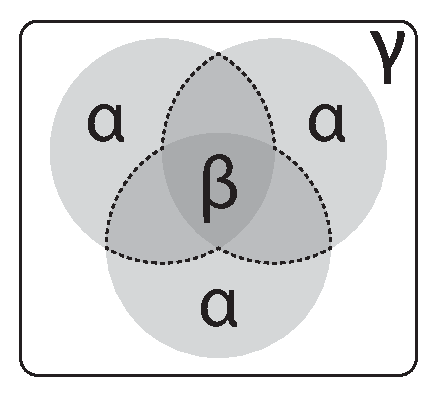
\includegraphics[width=0.4\textwidth]{./figures/Introduction/diversities}
  	\caption{Schematic representation of $\alpha$ (gray circles), $\beta$ (dotted line) and $gamma$ (blach square) diversities.\label{fig:diversities}}
\end{figure}
These indices are linked to the area of interest which can be of different sizes and, the habitats or the sites within it may vary their dimensions, accordingly. Both $\alpha$ and $\gamma$ diversities are subjected to the spatial scale chosen but no consensus has been reached on what spatial scales are appropriate to quantify these indices \cite{whittaker2001scale}. Therefore, it has been proposed that the definition of $\alpha$ and $\gamma$ diversities does not need to refer to a specific spatial scale: these indices can be measured for an existing environment of any size that consists of subunits at any scale. These scale-free definition is not applicable to $\beta$-diversity as it can not be calculated directly from species data \cite{tuomisto2010diversity}. Beta diversity in his original definition has to be considered as a measure of the species turnover between two sites \cite{whittaker1960vegetation}. The simplest definition of this index is: $\beta = \gamma/\alpha$; where gamma diversity is the total species diversity of a landscape, and alpha diversity is the mean species diversity per habitat. Here $\beta$-diversity quantifies how many subunits there would be if the total species diversity of the whole environment and the mean species diversity per sites remained the same, but the latter shared no species. Given these definitions of diversity measures, studying microbial populations in a particular environment requires the collection of ``samples'' able to inform us about the real natural diversity of that environment, but how can we estimate diversity?\\

\subsubsection{Diversity indices}
Several diversity indices have been used by researchers to quantify diversity, each one with its own characteristics and limits. One of the simplest diversity index is the so-called \textbf{species Richness} (usually noted, and here referred, as $S$), that is the number of different species detected in a given community. Although it gives a measure of the biodiversity of a particular environment, this index does not take into account any distribution parameter (like the relative abundance distribution of the species). In order to have a more detailed perspective of the biodiversity of a site others more complex indices have been developed considering species abundance data and probabilistic functions.\\

\subsubsection*{True diversity\label{par:tdiversity}}
This value is a measure of the effective number of types (or species); it refers to the number of equally-abundant types needed for the average proportional abundance of the types to equal that observed in the dataset of interest (where all types may not be equally abundant). The true diversity in a dataset is calculated by first taking the weighted generalized mean of the proportional abundances of the types in the dataset, and then taking the inverse of this \cite{tuomisto2010diversity}:
\begin{equation*}
{}^q\!D={1 \over \sqrt[q-1]{{\sum_{i=1}^S p_i p_i^{q-1}}}}
\end{equation*}
Here $p_i$ represent the proportional abundance of the $i$-th species, whereas $q$ is a ``sensitivity'' parameter that defines which kind of mean is used. With a sensitivity of 0 the mean corresponds to the weighted harmonic mean, which is 1/S because the $p_i$ values are removed. For a value of $q$ equal to 1 this equation is undefined and for a value equal to 2 the equation corresponds to the arithmetic mean. On the contrary, for increasing values of $q$ the generalized mean approaches the maximum $p_i$ value. In other words, $q$ modifies species weighting, such that increasing $q$ increases the weight given to the most abundant species. Consequently, for the same dataset, it is possible to obtain larger or smaller values of species diversity increasing or decreasing $q$, respectively. In case that all species are equally abundant, the value of $q$ has no effect on the diversity computation, which will be equal to the richness for every value of $q$.\\

\subsubsection*{Shannon-Wiener function}
The Shannon-Wiener function is one of the most popular diversity indices used in Biology and Ecology, even if its first definition was proposed independently by Claude Shannon and Norbert Wiener to quantify the entropy (uncertainty or information content) in strings of text \citep{shannon1949mathematical, wiener1948cybernetics}. this function has been called with a variety of names from Shannon-Weaver index (where Weaver refers to Wallace Weaver, Shannon's co-author) to Shannon entropy, but its correct definition is Shannon-Wiener function as reported in \citep{krebsj}. This index is based on the idea that more different species there are in a sample, and the more equal their proportional abundances are, the more difficult is to correctly predict the next randomly chosen species from the sample. It is most often calculated as follows:
\begin{equation*}
H' = -\sum_{i=1}^S p_i \ln p_i
\end{equation*}
let $p_i$ be the proportional abundance of the $i$-th species; this formula quantifies the uncertainty in predicting the species identity of an individual that is taken at random from the dataset. Historically, this equation is written using the natural logarithm, but it can be written freely choosing the base of the logarithm. Nevertheless, the most popular logarithmic bases are 2, 10 and e, corresponding to three different measurement units, which have been called binary digits (bits), decimal digits (decits) and natural digits (nats), respectively. Before comparing values of this index obtained with different logarithmic bases, it is required to convert them to the same logarithmic base and this can be done, as reported in Shannon work, multiplying one base for the log of the other base (for example if we want to change from the base $a$ to base $b$, this can be obtained with multiplication by $\log_{b}a$).\\
When all species found in a site of interest are equally common, all $p_i$ values equal $1/S$, and the Shannon-Wiener function takes the value $ln S$. The more unequal the abundances of the species, the smaller the corresponding Shannon entropy. Practically, if one species is very abundant, and the others are extremely rare (even if there are many of them), Shannon entropy approaches zero. In particular, if one site contains only one species, Shannon entropy exactly equals zero (in other words, there is no uncertainty in predicting the type of the next randomly chosen entity).\\
Another index similar to the Shannon-Wiener function is the \textbf{R\'{e}nyi entropy} \cite{alfred1960measures}. This index takes into account the same sensitivity parameter $q$ explained above in the~\nameref{par:tdiversity}~section. In particular, the R\'{e}nyi entropy is a generalization of the Shannon entropy to other values of $q$ than unity, and it can be expressed as:
\begin{equation*}
{}^qH = \frac{1}{1-q} \; \ln\left ( \sum_{i=1}^R p_i^q \right )
\end{equation*}
This expression can be written in another format:
\begin{equation*}
{}^qH = \ln\left ( {1 \over \sqrt[q-1]{{\sum_{i=1}^R p_i p_i^{q-1}}}} \right )
\end{equation*}
that is (see~\nameref{par:tdiversity}~section): 
\begin{equation*}
\ln({}^q\!D)
\end{equation*}

\subsubsection*{Simpson index}
This index was introduced for the first time by Edward H. Simpson in 1949 \cite{simpson1949measurement} for measuring the degree of concentration when individuals are classified into types. In Biology and Ecology this index is used to quantify the probability that two entities taken at random from the dataset of interest represent the same type. It is computed using the following formula: 
\begin{equation*}
\lambda = \sum_{i=1}^S p_i^2
\end{equation*}
In its original definition this index is more a measure of equality than diversity; in fact, the higher the value of this index, the smaller the number of different species in the dataset. Proportional abundances ($p_i$) are by definition constrained to values between zero and one, but their weighted arithmetic mean, and hence the Simpson index, can never be smaller than 1/S, which is reached when all types are equally abundant. As said before, since mean proportional abundance of the types increases with decreasing number of types and increasing abundance of the most abundant type, this index assumes small values in sites with high diversity and,
contrariwise, large values in sites with low diversity. This can be a counter-intuitive behaviour for a measure of diversity, so transformations of $\lambda$ that increase with increasing diversity have been often used. Two of the most popular of such transformations are the \textbf{inverse Simpson index} (defined as $1/\lambda$) and the \textbf{Gini–Simpson index} (defined as $1 - \lambda$) \cite{hill1973diversity,jost2006entropy}. It is worth noticing that both of these modification of the original Simpson index have been used in literature, usually referring to them as Simpson index, so care is needed to avoid accidentally comparing the different indices as if they were the same.\\

\subsubsection{The estimation problem}
Despite the high number of diversity indices and their different characteristics, all biologists who sample natural communities are plagued with the problem of how well a sample reflects a community's ``real'' diversity. Ecologists studying the diversity of macroorganisms have faced this estimation problem and have designed tools for dealing with the problem of sampling \cite{heck1975explicit, magurran1988ecological, colwell1994estimating}. The availability of microbial diversity data have increased the interest in applying these ``ecological'' tools to the microbial world. Several microbial studies have used diversity indices for comparing sample diversity, but their suitability is not completely clear \cite{mcmurdie2014waste}. Others new diversity estimators have been proposed in order to deal with microbiological data. However, the success of these tools has not yet been fully evaluated for microbial communities, and other approaches remains to be explored.\\
Estimating microbial diversity is not a trivial task and finding a way to compare how well this diversity has been estimated can be even harder. One possible way to face this problem is based on the assumption that in any community, the number of organism types detected increasing with sampling effort until all types are detected. The relation between the number of observed types and the sampling effort can be used as a possible measure of the total diversity of the sampled community. An accumulation curve is a possible way to inspect this relation simply plotting the cumulative number of types observed versus the sampling effort (as number of sampled units); in this way, differences in ``species diversity'' of the sampled community underlie differences in the shape of the curve. If the sampling effort is pushed to its maximum, the curve would eventually reach an asymptote representing the ``real'' number of different types in the observed community. In other words, the more concave-downward the curve, the better sampled the community. Another possible way to compare how well communities have been sampled is to plot their rank-abundance curves. In this plot, species are ordered from the most to least abundant on the $x$ axis; whereas the abundance of each observed species is plotted on the $y$ axis. Sample containing high number of rare species will produce a long right-hand tail; on the other hand, samples with a more equal distribution of species will generate plot with a very short right-hand tail (Figure~\ref{fig:accrank}).\\
\begin{figure}[!tb]
	\centering
	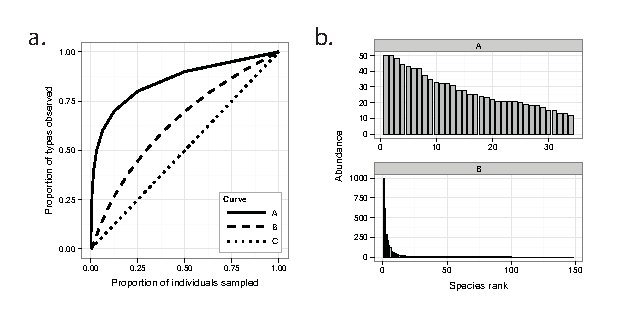
\includegraphics[width=\textwidth]{./figures/Introduction/rank_accumul1}
  	\caption{\textbf{a.} Accumulation curves. In the worst case scenario (C) is reported a linear curve indicating that every individual identified was a different type. On the contrary, in the best case scenario (A) the bacterial communities are well sampled and the samples therefore contain considerable information about the total richness as reflected by the concave-downward curve. The B scenario is a intermediate scenario between the other two. \textbf{b.} Rank-abundance plots. The samples in the panel A contain an equal distribution of species; whereas the samples in the panel B contain a large number of rare species resulting in a long right-hand tail of low abundance values.\label{fig:accrank}}
\end{figure}

\subsubsection*{Rarefaction analysis}
This statistical approach compares observed richness among different sites, treatments, or simply habitats that have been unequally sampled. A rarefaction curve results from averaging randomization of the observed accumulation curve (described above) \cite{foote1992rarefaction}. In particular, rarefaction curves are created by randomly re-sampling the pool of $N$ samples multiple times and then plotting the average number of types detected in each sample from 1 to $N$. As a consequence, rarefaction analysis is able to generate the expected number of species in a small collection of $n$ samples randomly drawing from the large pool of $N$ samples \cite{gotelli2001quantifying}. Normally, these curves grow rapidly at first (while the most common species are found), reaching a plateau as only the rarest species remain to be sampled. Let $N$ be the total number of items, $S$ the richness, $N_i$ the number of items in group $i$, and $M_j$ the number of groups consisting in $j$ elements; the rarefaction analysis is based on these assumptions:
\begin{equation*}
\sum_{i=1}^S N_i = N \hspace{10pt};\hspace{10pt} 
\sum_{j=1}^{\infty} M_j = K \hspace{10pt};\hspace{10pt}
\sum_{j=1}^{\infty} jM_j = N
\end{equation*}
If two sample with unequal $N$ have to be compared, it is possible to rarefy the biggest sample using a number of random sub-samples equal to the number of item in the smallest sample. In this way the size of biggest sample is virtually collapsed to the same of the smallest one, and the diversity of the two samples can now be compared.\\

\subsubsection*{Diversity estimators}
Given the fact that our knowledge of the natural world relies on samples; when we study the composition of microbial communities we have to find a way to inform us about the actual diversity of these microbial communities starting from the collected samples. Diversity estimators, as their name says, estimate the total diversity (richness) of a community form one or more samples. These estimators fall into three major classes: extrapolation from accumulation curves, parametric estimators, and non-parametric estimators \cite{hughes2001counting}. Curve extrapolation methods use the previously described accumulation curves, simulating an infinite sampling effort. In this way is possible to compute the total number of items in a sample by estimating the asymptote of the curve. In order for this method to work the simulated accumulation curve has to fit an assumed functional form; these model functions principally include Michaelis-Menten equation \cite{johnson2011original}, and the nagative exponential function. The advantage of estimating diversity through these methods is that once a species has been counted, there is no need to count it again; consequently, we can focus our attention on identify more rare species than collect again common ones. On the contrary, these methods are not suited for samples where only a small fraction of the total diversity has been identified. Here, curves fit equally well the models but their predicting power is very low (they have different asymptotes). Unfortunately, for microbial communities, is difficult to determine if the whole diversity has been well sampled, so this approach does not seem promising for estimating microbial diversity in most natural environments.\\
Parametric estimators are another class of estimation methods. These methods guess the number of unobserved species in a community by fitting collected data to relative abundance models. The most used abundance models for microbial community are: the log-normal model \cite{hill2003using, dumbrell2009relative}, and the Poisson log-normal model \cite{bulmer1974fitting, bohannan2003new}. Nevertheless, using parametric estimators for microbial communities has three main obstacles. First, data on relative species abundances are needed. These kind of data may be subjected to bias for microbial communities (counting microbial species in a community is not simple as already reported in this work). Second, they need a value of ``true'' abundance distribution, which can not be determined for microorganisms unless by fitting experimental data to a known pattern of distribution. Finally, even if one of the chosen models is a good approximation of the relative abundances of species in a community, these estimators require large data sets to correctly evaluate the distribution parameters, and this kind of data sets are not always available for microbial data.\\
The last class of estimators are the non-parametric estimators, which are the most used for microbial communities. These estimators have been adapted from the mark-release-recapture method (MRR) for estimating the size of animal population \cite{fletcher2006analysis}.
These methods are base on the assumption that the more the community is diverse the less probable is to ``recapture'' a ``marked'' and ``released'' species. In other words, in a very diverse community the probability to observe more than once the same ``marked'' species will be low; whereas in a depauperate community the same probability will be high. The MRR method is not suitable for microbiological data since marking, releasing and recapturing a microorganism is not possible. Derived methods that take into account the number of rare organisms have been developed to cope with this problem. The most used non-parametric estimators in biological literature are the \textbf{Chao1 index}, and the \textbf{abundance-based coverage estimator} (ACE), both based on an MRR-like ratio for estimating species richness \cite{chao1984nonparametric, chao1993stopping, sogin2006microbial, roesch2007pyrosequencing}. Chao1 index estimates the number of species in a community as:
\begin{equation*}
S_{Chao1} = S_{obs} + \frac{n_1^2}{2n_2}
\end{equation*}
where $S_{obs}$ is the number of detected species, $n_1$ is the number of species observed once (singletons), and $n_2$ is the number of species detected twice (doubletons). This index is very useful with microbial data sets because they tend to be skewed toward the low-abundance classes. In contrast with the Chao1 index, the ACE estimator incorporates data from species with less than 10 individuals; including them in this equation:
\begin{equation*}
S_{ACE} = S_{abund} + \frac{S_{rare}}{C_{ACE}} + \frac{F_1}{C_{ACE}} \gamma_{ACE}^2
\end{equation*}
here, $S_{rare}$ is the number of species with an abundance value smaller than or equal to 10 (rare species); whereas $S_{abund}$ is the number of species with an abundance value grater than 10 (abundant species). It is important to note that $S_{rare} + S_{abund}$ is equal to the total number of species detected in the sample. $C_{ACE}$ estimates the sample coverage in terms of species observed and is equal to:
\begin{equation*}
S_{ACE} = 1 - \frac{F_1}{N_{rare}}
\end{equation*}
where $F_1$ is the number of species with with only one individual and $N_{rare}$ is:
\begin{equation*}
N_{rare} = \sum_{i=1}^{10} iF_i
\end{equation*}
with $F_i$ the number of species with $i$ individuals. The last term to be defined is $\gamma_{ACE}^2$, which estimate the coefficent of variation of $F_i$ and is defined as:
\begin{equation*}
\gamma_{ACE}^2 = max\left[\frac{S_{rare}\sum_{i=1}^{10} i\left(i-1\right)F_i}{C_{ACE}\left(N_{rare}\right)\left(N_{rare}-1\right)} - 1, 0\right]
\end{equation*}
It is worth noticing that both Chao1 and ACE underestimate the true diversity richness for low sample sizes. For example, the maximum value of $S_{Chao1}$ is $(S_{obs}^2 + 1)/2$ when one species in the sample is a doubleton and all others are singletons. Thus, $S_{Chao1}$ will strongly correlate with sample size until S obs reaches at least the square root of twice the total richness.\\
Despite these methods for studying microbial diversity there is still no method universally accepted. Further work is needed in order to fully evaluated the existing indices and to develop new and more feasible ones for microbial studies. Ideally, with the increasing interest in new sequencing technology and the generation of larger data sets of microbial data will be possible to better evaluate both biases and precision of diversity estimators. Augmenting this new technology  with statistical approaches obtained from ``macro'' studies could offer a powerful means to study the ecology and the evolution of microbial species in natural environments.

\subsection{An intertwining of languages: the microbiome}
As already said, biologists have long appreciated the roles played by microorganisms in two distinct fields of pathogenesis and ecosystem cycling. Studies of bacteria hosted by human body started with Antonie van Leeuwenhoek in 1680s. He compared microorganisms from fecal and oral samples of healthy and ill individuals revealing striking differences between the observed groups (both between the two districts of the human body and between the two different conditions of the individuals) \cite{van1684abstract, dobell1920discovery}. In more recent times, the interaction between microbes and plants has been intensively explored shading light on new possible methods of cultivation and defining groups of microorganisms associated with plant health \cite{lundberg2012defining}. In the last two decades, the widespread application of genetic and genomic approaches has revealed a bacterial world astonishing in its diversity and complexity. These new technologies have provided researchers with microbial data from the most different organisms (from the human body to the ant gut) altering our understanding of macroorganisms biology.\\
In 2001 Joshua Lederberg coined the term microbiome referring to ``the ecological community of commensal, symbiotic, and pathogenic microorganisms that literally share our body space'' \cite{lederberg2001scientist}. As time passes, the term ``microbiome'' has been referred to other types of macroorgansims such arthropods, fish, and plants. Many studies have been performed in animals and plants, reporting the description of the bacterial communities (microbiome) found in several districts as gut, roots, skin, and leafs \cite{hyde2013living, stoll2007bacterial, ilmberger2014comparative, ringo2006characterisation, berlec2012novel}. Currently, many scientific articles distinguish ``microbiome'' and ``microbiota'' to describe either the collective genomes of the microorganisms that reside in an environmental niche or the microorganisms themselves. However, by the original definitions, these terms are largely synonymous.\\
Microorganisms have found to play a central role in plant differentiation and activity. Indeed, they supply plants with nutrients, play a central role in the establishment and the development of root systems. In addition, microorganisms are able to protect plants against pathogens and other environmental stress conditions. It is estimated that more than 10'000 different species of plants are dependant on microbial activity for development, growth, and survival \cite{van2008unseen}. Studies on the microbial hosts of plants have been focused in three main locations: the rhizosphere (immediately surrounding the root) \cite{borruso2014rhizosphere}, on the leaves \cite{rastogi2012leaf}, phyllosphere (fruits and flowers) \citep{aleklett2014microbial}, and inside plant cells (endophytes) \cite{bulgarelli2013structure}. Microorganisms in the rhizosphere are selected based on both their functional abilities and their taxonomy \cite{singh2004unravelling}. Here, root-derived rhizodeposits supply organic substrates which, in turn, shape bacterial communities selecting host-specific bacterial assemblages (the microbiota) \cite{bulgarelli2013structure}. Indeed, it has been shown that plant’s specific exudates are major contributors to the plant specificity of rhizosphere microbiota \cite{berg2009plant}. Large populations of microorganisms also live in the phyllosphere. Here, several conditions, like extreme temperatures, dryness, irradiation, oxidative stress, and poor nutrient availability, are able to modify bacterial communities and, consequently their activity \cite{lindow2003microbiology}. Interestingly, similarly to the human gut, these species belong to a small number of dominant phyla, including \textit{Actinobacteria}, \textit{Bacteroidetes}, \textit{Firmicutes}, and \textit{Proteobacteria} \cite{redford2010ecology}. This phenomenon is in accordance with the special conditions known to occur in the interaction between microbes and their host, resulting in a specific adaptation and activity.\\
Based on molecular and cellular data, animals and choanoflagellate protists are now considered sister groups, descended from a common choanoflagellate-like ancestor \cite{carr2008molecular}. Homologous of animal signaling and adhesion proteins have been found in choanoflagellates; these proteins may have developed as critical facilitators of bactivory \cite{nichols2009genomic}. Moreover, some animals are able to respond to bacterial signals as triggers for morphogenesis or behavior. Therefore, the discovery that at least one choanoflagellate, \textit{Salpingoeca rosetta}, responds to signals from specific bacteria to initiate colony formation through cell division hints at an ancient involvement of bacteria in the initiation of multicellularity \cite{alegado2012bacterial}. As animals diversified, the interactions between animals and bacteria continued shaping their evolution. Bacteria took on a new role in animal nutrition, serving not only as prey but also as producers of digestible molecules in the animal gut. The evolution of gut itself was certainly influenced by bacteria. The advent of the coelom made gut elongation and regional specialization possible, facilitating both massive ingestion and storage for later digestion. Although the degree to which microbes have driven gut evolution is unknown, the radiation of several animal groups was undoubtedly enabled by alliances with their gut-associated microbiota (e.g. ruminants). The animal evolution has also influenced the distribution and diversification of bacteria promoting the proliferation of bacterial species exclusively in particular animals \cite{hongoh2010diversity}. However, such specialization, comes with a cost: for every animal species that goes extinct, an unknown number of unique bacterial lineages that have evolved to depend on this animal niche disappear as well \cite{staley1997biodiversity}. On a wider scale, the evolution of animals provided new environments for bacterial colonization (e.g. deep sediments resulting from animal burrowing). Finally, human activities, which produce a range of xenobiotic molecules, have driven selection on bacterial catabolic pathways, leaving a signature of our presence in microbial metabolism \cite{janssen2005bacterial}.\\
The genomes of macroorganisms and microorganisms are reflecting their ancestral alliance. The analysis of the available genomes has revealed that most life forms share approximately one third of their genes, including those encoding central metabolic pathways \cite{domazet2008ancient}. Not surprisingly, many animal and plant genes are homologs of bacterial genes, mostly derived by descent, but even by gene transfer from bacteria \cite{keeling2008horizontal, hemmingsen1988homologous, pear1996higher}. Many arthropods have intracellular bacterial symbionts able to provide them with novel metabolic capabilities (synthesis of essential amino acids, photosynthesis, or chemosynthesis) \cite{andersson2006genetics}. Certain marine invertebrates maintain algal plastids as photosynthetically active symbionts, allowing them to use photosynthesis as a food source for extended periods \cite{rumpho2011making}. These metabolic additions allow the animal to thrive by adapting to otherwise noncompetitive lifestyles or environments \cite{dubilier2008symbiotic}. Microbial communities in the gut of vertebrates respond to the host diet endowing animals with the flexibility to digest a wide variety of molecules \cite{ley2008worlds, muegge2011diet}.\\
These findings have been the starting point for the development of new theories in multiple fields of biology from immunology \cite{round2009gut} to evolutionary biology \cite{mcfall2013animals}. On the other hand, these new data need a reexamination of the concepts of what constitutes a genome, a population, an environment, and an organism. Similarly, features once considered sporadic or exceptional, are now demonstrated to be able to drive the evolution of macroorganisms, leading to the advent of novel biology models. In particular, microbiology, presents hard challenges both to the species concept, as formulated by Ernst Mayr in 1942, and to the concept that vertical transmission of genetic information is the only motor of selectable evolutionary change.\\

\subsubsection{The hologenome theory of evolution}
This theory, proposed for the first time by Eugene Rosenberg at al. in 2007 \cite{rosenberg2007role}, defines a new biological entity composed by both a host (macroorganism) and a multitude of hosted organisms (microbiota). This entity (called ``holobiont'') has a genome which consists in the sum of the genetic information of the host and its microbiota; this genome has been called the ``hologenome''. Following this theory, the holobiont with its hologenome has to be considered as a single unit of selection in evolution capable to adapt to rapid changes in environmental conditions. The evolution of this entity can occur by changes in the host genome and/or in any of the associated microbial genomes, and relies on cooperation between the genomes within the holobiont, as much as on competition with other holobionts. The hologenome theory of evolution was first discussed using bacterial blenching of corals as model. Despite corals possess a restricted specific immune system they became resistant to the infection of a specific pathogen, \textit{Vibrio shiloi}. In their work, Rosenberg and his collaborators, presented the coral probiotic hypothesis, stating that a dynamic relationship could exist between symbiotic microorgansims and corals under different environmental conditions.\\
The hologenome theory is based on 4 generalizations:
\vspace{-5mm}
\begin{itemize}[nosep]
\item Animals and plants establish symbiotic relations with microorganisms
\item Symbiotic microorganisms can be transmitted between generation
\item Host-microbiota association affect the fitness of the holobiont in the environment
\item Genetic variation in holobionts can be enhanced by incorporating different microbial populations and can change rapidly under different environmental conditions
\end{itemize}

\paragraph{Animals and plants establish symbiotic relations with microorganisms}
Culture-free DNA based techniques have permitted to inspect the vast majority of microorgansims on or in animal and plant tissues. As a consequence, several interesting generalizations have emerged. First, the diversity of microorganisms hosted by a particular animal or plant species is very high. Second, the host-associated community is very different from that found in the surrounding environment \cite{chelius2001diversity, sharp2007vertical}. Third, similar microbial populations are found on the same species in different geographic areas; whereas, different populations are found on different species at the same location \cite{rohwer2002diversity, lambais2006bacterial}.  Next, Different microbial communities often dominates different tissues of the same organism. Finally, only certain bacterial groups are found in particular tissues even if a large diversity exists (e.g. the human gut has been reported to contain more than 1000 bacterial species \cite{rajilic2007diversity}, but only two divisions, Bacteroidetes and Firmicutes, make up 99\% of the total bacterial population \cite{ley2006ecological}).\\
The association between microorganisms and host can take many different forms. Some microorganisms are able to establish transitory interactions with their host; whereas, on the opposite side, there are some interactions that can lead to total dependence of one on the other. Between this two extremes there is a gradient of associations of varying strengths regulated by mechanism able to either increase or reduce the diversity of the hosted microbiome. One of the factor that determine the diversity of microorganisms associated with the holobiont is the variety of different niches that can change during changing phases of the host. Every time that the conditions of a particular niche changes a diverse microbial community is established, with different microbial strains thriving in the new conditions. This diversity may allow the holobiont to function more optimally and adapt more rapidly to changing conditions (this effect has been called the ``insurance policy hypothesis'' \cite{yachi1999biodiversity}). Even bacteriophages contributes to increase bacterial diversity of the holobiont. If any microorganism becomes too abundant, the bacteriophages present in the host tissues kill it re-establishing the equilibrium of the community (this concept has been called ``kill the winners'' hypothesis \cite{thingstad1997theoretical}).\\
On the other side, one force is able to limit the number of strains that are allowed to survive and become established in the holobiont: the immune system of the host. Plants have evolved myriad phytochemicals, whose purpose is to prevent infections by harmful microorganisms and enable coexistance with beneficial ones. Organisms with innate and adaptive immune systems are able to recognize ``foreign'' microorganisms and generate an immune response capable of eliminating these microbes. The immune system of the host is responsible for both limiting the number of types of microorganisms that can survive within the holobiont and recognizing and accommodating the normal microbiota. It is worth noticing that some resident symbiotic bacteria are also part of this system by occupying potential adhesion sites and by producing antibiotics \cite{ritchie2006regulation}.\\

\paragraph{Symbiotic microorganisms can be transmitted between generation}
The holobiome theory is based on the continuity of partnership between new generations. Therefore, both host and symbiont genomes must be transmitted from one generation to another. The vertical transmission of the host genome from parents to children is achieved in various through sexual reproduction and other well defined mechanisms. In recent years it has become clear that even microbial symbionts can be transmitted through generations by a large variety  of methods. One method of transmission is direct transmission which occurs with symbionts where microorganisms are in or on the reproductive cells. An extreme case of direct transmission is represented by mitochondria and chloroplasts, which can be considered as symbionts that are directly transmitted by cytoplasmic inheritance. Another method of transmission is direct contact. Here, symbionts are derived during passage through the birth canal or subsequently by physical contact with parent or family and community members. There also other less direct modes of transmission reported in literature; for examples (see Table \ref{tab:transm}).
\begin{table}
\centering
\scriptsize
\begin{tabular}{ p{0.2\textwidth} p{0.28\textwidth} p{0.28\textwidth} p{0.1\textwidth} }
\hline
Holobiont : Microbiota & Mode of transmission & Microbial contribution & References \\ \hline \hline
Termite : Microbiota in hind gut & Feces of adult termites fed to newly hatched juveniles & Utilizable energy and carbon; nitrogen metabolism; recognition signal from odor of bacterial metabolites & \cite{abe2000termites, minkley2006nest} \\
Squid nidamental gland : Microbiota & Via cover of eggs originating from the gland & Protection of eggs and embryos against pathogens & \cite{kaufman1998bacterial, barbieri2001phylogenetic} \\
Corals : Microbiota & From the environment and by vegetative reproduction & Photosynthesis (intracellular algae); nitrogen fixation; protection against pathogens & \cite{rohwer2002diversity, buddemeier2004adaptive, rosenberg2007role} \\
Sponges : Microbiota & Environmental in addition to possible transmission from parent & Breakdown of complex polymers; nitrogen cycling; protection against pathogens & \cite{webster2001phylogenetic, hickman2005have, taylor2007sponge} \\
Cow rumen : Microbiota & Physical contact with parents and via food contaminated with feces and sputum & Provision of all nutritional needs from cellulose & \cite{dehority2003rumen, russell2001factors} \\
Human gut and mouse model : Microbiota & Via physical contact and from environment & Protection against pathogens; stimulation of immune system; angiogenesis; vitamin synthesis; fiber breakdown; fat storage & \cite{hooper2002host, o2006gut, ley2006ecological, xu2007evolution} \\
Land plants : Mycorrhiza fungi & Via seeds on ground and by vegetative reproduction & Supply of minerals from soil & \cite{wilkinson2001mycorrhizal, wang2006phylogenetic} \\
Legume plants : Rhizobium & Environmental from surrounding & Nitrogen fixation & \cite{stougaard2000regulators, jones2007rhizobial} \\
Plant : Growthpromoting rhizobacteria & Environmental from surrounding soil & Protection against pathogens; nitrogen metabolism; acceleration of mineralization; carbon cycling; salt tolerance & \cite{smith1999genetic, somers2004rhizosphere, singh2004unravelling} \\
\hline
\end{tabular}
\caption{Modes of transmission of symbionts and their contribution to the fitness of the holobiont (adapted from \cite{zilber2008role}) \label{tab:transm}}
\end{table}
The large variety of transmission modes implies that individuals can acquire and transmit symbionts during each moment of their life and not just during their reproductive phase. As a consequence, any organism in close contact with an offspring is able to transfer microbes influencing the holobiont of the next generation.\\

\paragraph{Host-microbiota association affect the fitness of the holobiont in the environment}
As reported in Table~\ref{tab:transm}, there are several representative symbiotic systems that contribute to the fitness of the holobiont. In more extreme cases, neither the host nor the symbiont can survive without the other, a phenomenon called ``absolute mutualism''. Regardless of the extent of dependency, microorganisms play numerous roles in metabolism, regulation, disease resistance and is sex and fertility determination of their hosts. For example, the microbial imbalance (dysbiosis) in the human gut may predispose to pathogen proliferation which, in turn, increases non-specific inflammation. This situation may predispose certain genetically susceptible people to inflammatory disease and may be caused by pathogens, which are opportunistic organisms that cause acute inflammation \cite{round2009gut} (see Figure~\ref{fig:dysb}).\\
\begin{figure}[!tb]
	\centering
	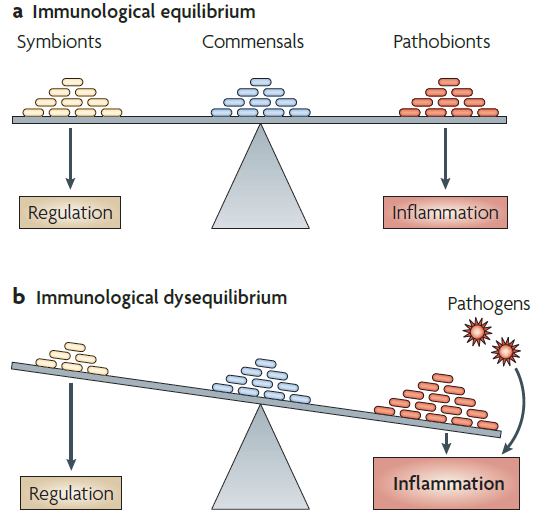
\includegraphics[width=0.6\textwidth]{./figures/Introduction/gut_dysbiosis}
  	\caption{Immunological dysregulation associated with dysbiosis of the microbiota. a) A healthy microbiota with a balanced bacterial composition. Pathobionts are permanent residents of the microbiota and have the potential to induce pathology. b) Dysbiosis condition: an unnatural shift in the composition of the microbiota, which results in either a reduction in the numbers of symbionts and/or an increase in the numbers of pathobionts (from \cite{round2009gut}). \label{fig:dysb}}
\end{figure}
Another example is the bovine rumen which is able to act like an anaerobic fermentator inducing the proliferation of suitable bacteria for converting the cellulose into its glucose subunits. This subunits are then fermented by other different groups of bacteria to produce short-chain fatty acids which are absorbed through the wall of the rumen into the bloodstream \cite{dehority2003rumen}. The bovine holobiont benefits from this cooperation by being able to grow and reproduce on a simple diet of cellulose, water and inorganic salt, resulting in an increased fitness of the whole holobiont. Following these examples, it is possible to notice the very tight and complex interactions occurring within the holobiont between the host and its microbiota, supporting the reference to the microbiota as an ``additional organ''.\\

\paragraph{Genetic variation in holobionts}
The dual nature of the holobiont reflects a pool of genetic variation due to both the host genome and the symbiont genome. Variations in host genome may occur during sexual reproduction, chromosome rearrangements, and, ultimately by mutations. Even the genome of the microbiota may vary during conjugation, transduction, and DNA transformation.  In addition to these processes, changes in the genome of the microbiota can occur by three other mechanisms: microbial amplification, acquisition of novel strains and horizontal gene transfer between different species. These processes can occur very rapidly under environmental demand and may be crucial element for the evolution of the holobiont.\\
Microbial amplification is the most rapid mode of variation. It involves changes in the abundance of the diverse types of associated microorganisms that can occur as a result of modifications in the environmental conditions (temperature, pH, nutrient availability etc...). Considering the large amount of genetic information encoded in the diverse microbial population of holobionts, microbial amplification is a powerful mechanism for adapting to different environmental conditions.\\
Acquisition of new symbionts from the environment is another important mechanism of genetic variation. Animal and plants are constantly in contact with billions of microorganisms during their lifetime. Occasionally, one of these organisms may become established in the host finding a suitable niche. Under the appropiate conditions this novel individual may become more abundant and affect the phenotype of the holobiont . Acquiring new strains can introduce entirely new genese into the hologenome of the holobiont, leading to the acquisition of peculiar characteristics previously unavailable.\\
Horizontal gene transfer between the host microbiota is an additional potent mechanism for generating variability. This process is driven by trasposons, plasmids, bacteriophages and genomic islands, which can be either on the bacterial chromosome or on the plasmids. The evolutionary significance of horizontal gene transfer is that an entire block of DNA can be transferred from one bacterium to another in a single step. This has resulted in a rapid evolution of diverse strains of nitrogen-fixing mesorhizobia in legumes \cite{nandasena2007situ}. If the environmental conditions changes rapidly, the host genome alone may not evolve quickly enough and the organism may lose competitiveness. Rapid changes in the symbiont microbiota could allow the holobiont to adapt and survive even during an increase selective pressure.\\

\section{Two sides of the same coin: from Genomics to Metagenomics}
One approach that has contributed to the comprehension of both microscopic and macroscopic organisms is genomics. Through genomics, researchers have become able to learn about the evolution and capabilities of organisms by deciphering their genome (the genetic material of an organism). Genomics has also greatly advanced microbiology, but, like pure culture, traditional genomics is limited in its ability to elucidate the dynamics of microbial communities. Given the evidence that many microbes resist being cultured, culture-independent methods for identifying and characterize microbes in the environment have come to play a larger and larger role over the last several decades. Starting from 1980 the idea to inspect whole microbial communities by sequencing the genetic material collected directly from the environment became more and more popular. The decreasing DNA sequencing cost ensured an increasing interest in this application of biology leading to the birth of ``metagenomics'' as a separate discipline. Currently, both disciplines are coexisting, complementing each other to provide new insights into microbial communities and activities that control matter and energy flux on Earth and that are able to interact with macroscopic organisms. Indeed, Metagenomics provides a means for studying microbial communities in their complexity without the need to isolate a single strain. Moreover, complex ecological interactions (as lateral gene transfer, phage-host dynamics, metabolic complementation etc...) can now be inspected through the lens of metagenomics. On the other hand, Community composition, function, and dynamics can now be measured and modeled in the environment with universal microbial-community genomic approaches. With such information in hand, it will become possible to interpret the microbial dynamics between natural cycles and human activities that together shape the future of the planet.\\

\subsection{Genomics and the role of DNA sequencing\label{par:genomics}}
Following Rosalind Franklin's confirmation of the helical structure of DNA around 1941 \cite{maddox2012rosalind}, in 1953 James D. Watson and Francis Crick's publicated the chemical structure of DNA \cite{watson1953molecular}. These findings paved the way for the Fred Sanger's publication of the amino acid sequence of insulin two years later \cite{sanger1953amino}. In 1965, Robert W. Holley and colleagues published the first DNA sequence ever determined, the alanine transfer RNA \cite{holley1965nucleotide}. After this work, Marshall Nirenberg and Philip Leder revealed the triplet nature of the genetic code and were able to determine the sequences of 54 out of the existing 64 codons with their experiments \cite{nirenberg1965rna}. In 1972, Walter Fiers and his team determined the first sequence of a gene: the gene for Bacteriophage MS2 coat protein \cite{jou1972nucleotide}. From the early 1980s the idea of sequencing the genome of our own species began to be discussed and was seriously considered at federally sponsored workshops in 1984 and 1985 \cite{lambright2002managing}. After the improvements in sequencing technologies, nucleic acid sequencing became a major target of early molecular biologists.\\
The advent of DNA sequencing technologies led to a dramatical intensification of the completion speed of genome sequencing projects. The sequence of the first complete genome was that of the human mitochondrion (16'568 bp, about 16.6 kb); it was reported in 1981 \cite{anderson1981sequence}, five years before the complete sequence of the first chloroplast genomes \cite{shinozaki1986complete}. In 1992, the chromosome III of brewer's yeast Saccharomyces cerevisiae (315 kb) was sequenced \cite{oliver1992complete}. The first genome of a free-living organism sequenced was that of Haemophilus influenzae (1.8 Mb) in 1995 \cite{fleischmann1995whole}. In the following year a consortium of researchers from laboratories across North America, Europe, and Japan announced the completion of the complete genome sequence of an eukaryote, again Saccharomyces cerevisiae (12.1 Mb). In 2000, the Human Genome Project (HGP) has been completed publishing the first sequence of all the chromosomes composing the human genome \cite{collins1998new}. This project has opened a new field of biology not only for studying the human body and its characteristics but also for microbes. Questions first asked at the level of individual molecules and genes have better and more complete answers at the level of genomes and systems. It is now nearly unthinkable to launch a major comprehensive initiative in the biology of any species without sequencing its genome. Currently, the GeneBank database contains a huge amount of complete genome data from all over the world, including 4'432 virus, 29'260 archaea and bacteria and 1'775 eukaryote genomes (Figure~\ref{fig:numseq}).\\
\begin{figure}[!tb]
	\centering
	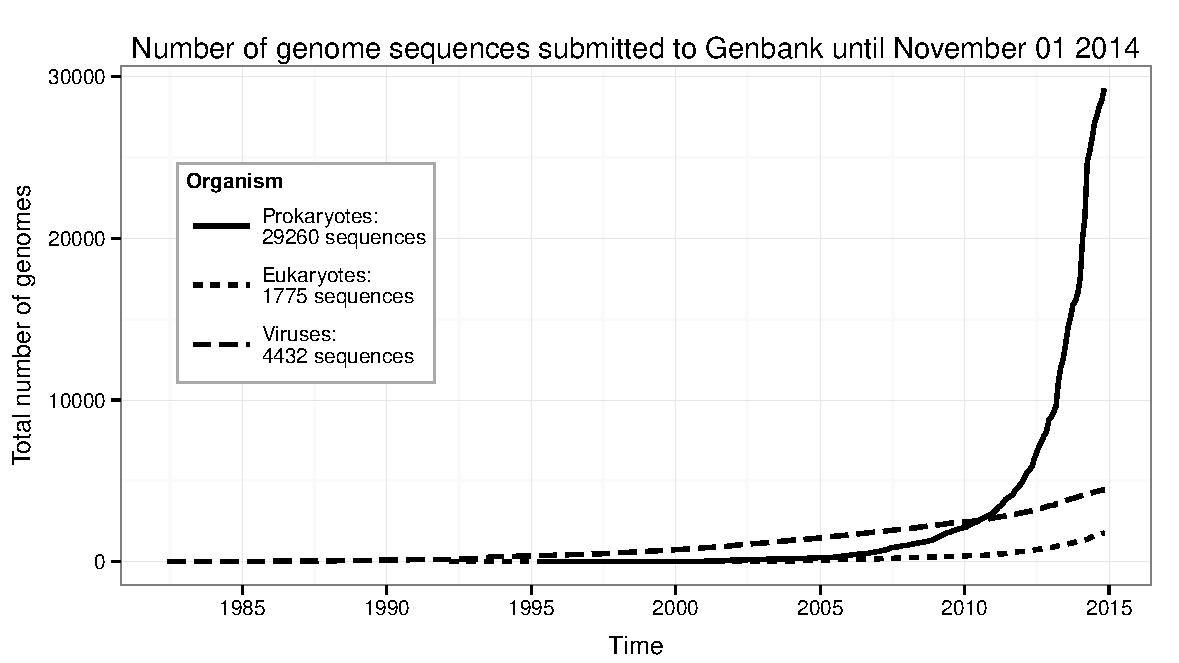
\includegraphics[width=0.9\textwidth]{./figures/Introduction/seq_number_genebank}
  	\caption{The number of genome projects has increased as technological improvements continue to lower the cost of sequencing. Exponential growth of genome sequence databases (GeneBank) since 1995. \label{fig:numseq}}
\end{figure}
In the light of this big amount of data, it is possible to define all the steps involved in the design of a genomic project in its most general form. Commonly, a genomic process consists of four step:
\vspace{-5mm}
\begin{enumerate}[nosep]
\item Selection and isolation of the organism of interest
\item Sequencing of the DNA extracted from pure cultures
\item Assembly of the generated sequences to create a representation of the original chromosome/s
\item Annotation and analysis of the obtained representation
\end{enumerate}
\textbf{Selecting} and \textbf{isolating} a microorganism is not a trivial task. In 1985, Staley and Konopka reviewed data on the cultivation of microbes from environmental samples under standard laboratory conditions \cite{staley1985measurement}. They defined what was called the ``great plate-count anomaly'': the vast majority of microbial cells that can be seen in a microscope cannot be induced to produce colonies on Petri plates or cultures in test tubes. Currently, it is estimated that only 0.1-1.0\% of the bacterial calls present in soil can be cultured under laboratory conditions; the culturable fraction of bacteria from aquatic environments is ten to a thousand times lower still \cite{kirk2004methods, oliver2005viable}. It is worth noticing that the fraction of organisms cultivatable in isolation will likely always be low, since, for growing it takes a community. Culturing always favours the recovery of organisms that are best able to thrive under laboratory conditions, usually neither the dominant nor the most influential organisms in the environment.\\
\begin{figure}[!tb]
	\centering
	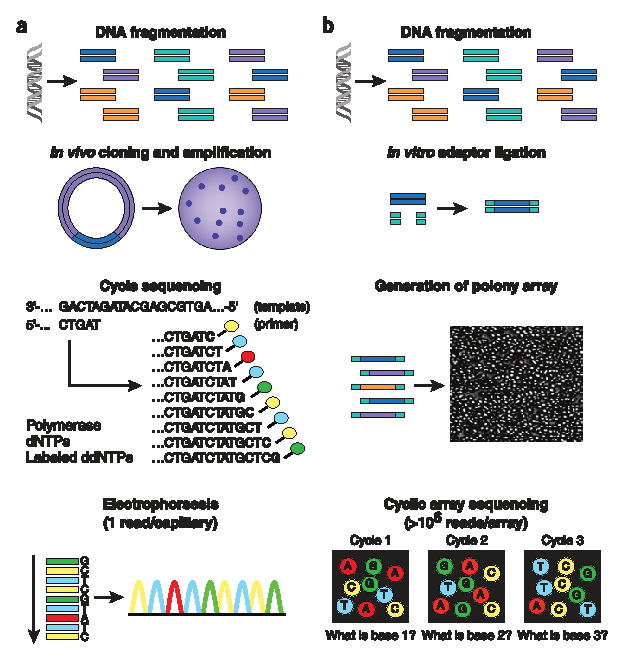
\includegraphics[width=0.7\textwidth]{./figures/Introduction/seq_approaches}
  	\caption{Work flow of shotgun versus next-generation sequencing. (a) With shotgun Sanger sequencing, genomic DNA is first fragmented, then cloned into a plasmid vector used for transforming a host (generally E. coli). A ladder of ddNTP-terminated, dye-labeled products, are generated and then subjected to high-resolution electrophoretic separation. As fragments pass a detector, the four-channel emission spectrum is used to generate a chromatogram which will be successively transformed into a set of DNA sequences. (b) In shotgun sequencing with cyclic-array methods, common adaptors are ligated to fragmented genomic DNA, which is then subjected to one of several protocols that results in an array of millions of spatially immobilized PCR colonies. Each colony (or ``polony'') consists of many copies of a single shotgun library fragment. As all polonies are tethered to a planar array, they can be sequencied in parallel. Similarly, the detection of fluorescent labels, incorporated with each extension, can be used to acquire sequencing data on all features in parallel. Multiple iterations of syntesis and imaging are used to build up a contiguous sequencing read for each array (from \cite{shendure2008next}). \label{fig:seqappr}}
\end{figure}
\textbf{Sequencing the DNA} of a ``pure'' organism can be done with several different technologies each one with its own characteristics. Despite the availability of a large set of sequencing machines, genome sequencing approaches fall into two broad categories, shotgun and high-throughput (next-generation or second-generation) sequencing. Since the early 1990s, DNA sequence production has almost exclusively been carried out with capillary-based, semi-automated implementations of the Sanger biochemistry today's called \textbf{shotgun sequencing}. In these methods, the sequencing biochemistry takes place in a ``cycle sequencing'' reaction, in which cycles of template denaturation, primer annealing and primer extension are performed multiple times until the DNA sequence of interest has been entirely sequenced. The Sanger biochemistry has been gradually improved since its first publication almost thirty years ago. Currently, it can be applied to achieve a read length of up to 1'000 bp, and per-base accuracies of \textasciitilde99.999\% with a sequencing costs of \$0.50 per kb. On the other hand, the term \textbf{next-generation sequencing} refers to all the different implementations of the so-called cyclic-array sequencing \cite{margulies2005genome} that have recently been realized in a variety of commercial products (e.g. 454 sequencing , Solexa technology, the SOLiD platform and the HeliScope Single Molecule Sequencer technology). The sequencing process itself involves alternating cycles of DNA sequence synthesis and imaging-based data acquisition. The enzyme driving the synthesis of DNA can be either a polymerase or a ligase; whereas data are acquired by imaging of the full array at each cycle. These array-based sequencing techniques enables a much higher degree of parallelism than conventional capillary-based used sequencing dramatically reducing the costs for DNA sequence production (read length, per-base accuracy and costs per kb vary between the different NGS implementations). Despite this great amount of different sequencing approaches and technologies, an election method for DNA sequencing does not exist but it depends on the project that has to be done and the money that a laboratory can afford.\\
\begin{table}
\centering
\scriptsize
\begin{tabular}{ r c c c c }
\hline
\textbf{Name} & \textbf{Cost (Mb)} & \textbf{Cost (Instrument)} & \textbf{Read-length (bp)} & \textbf{Reference} \\ \hline \hline
454 & \$60 & \$500'000 & 250 & \cite{margulies2005genome, dressman2003transforming} \\
Solexa & \$2 & \$430'000 & 36 & \cite{bentley2006whole, fedurco2006bta} \\
SOLiD & \$2 & \$591'000 & 35 & \cite{shendure2005accurate, mckernan2013reagents} \\
Polonator & \$1 & \$155'000 & 13 & \cite{shendure2005accurate, dressman2003transforming} \\
HeliScope & \$1 & \$1'350'000 & 30 & \cite{harris2008single, braslavsky2003sequence} \\
\hline
\end{tabular}
\caption{Principal characteristics of the most common NGS platfroms. Cost per Mb and instrument cost are to be considered as approximative (adapted from \cite{shendure2008next}). \label{tab:ngs}}
\end{table}
As reported above, the current DNA sequencing machines cannot read whole genomes as a continuous sequence, but rather read small pieces of between 20 and 1000 bases, depending on the chosen technology. These fragments must be aligned and merged in order to reconstruct the original DNA sequence, a process called \textbf{sequence assembly}. Assembly can be broadly categorized into two main approaches: \textit{de novo} assembly and comparative assembly \cite{pop2009genome}. The first method implies the assemblage of the sequence fragments obtained without the aid of a reference genome. The native version of this method is very complex and time consuming since the assembly algorithm needs to compare every read with every other read that has to be assembled (an operation that has a time complexity of $O\left(n^2\right)$) making it less favourable for short reads obtained with NGS technologies. However, more recent implementations of this algorithm uses an approach based on the ``De Bruijn graph'' drastically reducing the complexity of the algorithm and making it more affordable for NGS sequences \cite{compeau2011apply}. The second method, implies assembling reads against an existing backbone sequence, resulting in a sequence that is similar but not identical to the chosen backbone. Normally, the backbone sequence used is chosen from a set of existing sequence of a closely related organism in order to prevent misleading joints due to an high taxonomic distance. A common assembly pipeline involves the utilization of both methods using the first one for assembling newly generated sequences into bigger DNA fragments (scaffold) and then using the second one to join the generated fragments together.\\
The last step of a genomic pipeline consist in the \textbf{annotation and analysis} of the generated sequences. Genome annotation is the process of attaching biological information to DNA sequences; it consists of three main steps: $i)$ identifying portions of the genome that do not code for proteins, $ii)$ identifying elements on the genome (gene prediction) and $iii)$ attaching biological information to these elements. There are several automatic annotation tools to perform these steps \textit{in silico}, as opposed to manual annotation (curation) which involves human expertise and experimental verification. Ideally, these approaches complement each other in the same annotation pipeline. Normally, the basic level of annotation is performed using tools suited for finding similarity between sequences and then annotating genome based on homolouges \cite{altschul1990basic, langmead2012fast}. These tools use a reference sequence (the query sequence) to compare it with other DNA sequences stored in a biological database. Some databases use genome context information, similarity scores, experimental data, and integrations of other resources to provide genome annotations; whereas others rely on both curated data sources as well as a range of software tools in their automated genome annotation pipeline \cite{flicek2012ensembl}.\\
The analysis of a genome is not trivial and can, in turn, be composed of multiple analyses involving different research areas of genomic. Dynamic aspects of an organism, such as gene transcription, translation, and protein–protein interactions, can be explored through ``Functional genomics'' which attempts to answer questions about the function of DNA at the levels of genes, RNA transcripts, and protein products \cite{king2004functional}. The genomic branch aiming to obtain the 3-dimensional structure of every protein encoded by a given genome is called ``Structural genomic'' which allows the determination of protein structure by a combination of experimental and modeling approaches \cite{brenner2000expectations}. The principal difference between structural genomics and traditional structural prediction is that structural genomics attempts to determine the structure of every protein encoded by the genome, rather than focusing on one particular protein. Moreover, It is possible to identify reversible modifications on a cell’s DNA that affect gene expression without altering the genomic sequence (``epigenetic modifications''). These modifications include DNA methylation and histone modification which play an important role in gene expression and regulation (they are involved in numerous cellular processes such as in differentiation/development and tumorigenesis) \cite{jones2002fundamental}. Finally one of the most recent branch of genomic is \textbf{Metagenomics}. This approach aims to study the ``metagenomes'' namely the  genetic material recovered directly from a set of samples. Samples can be collected from the most different environments including host tissues, polluted soils, aquatic environments and many many more. Currently, Metagenomics is becoming a new science on its own comprising many approaches and methods specifically designed to cope with all the problems related to the study of bacterial communities as a whole.\\

\subsection{A community perspective: thinking meta}
The term ``meta'' is a Greek term that means ``transcendent''. The use of this suffix in the word metagenomics reflect the main goal of this science: understand biology at the community level \textit{transcending} the individual organism by focusing on collective genes and how they might influence each other’s activities in serving shared functions. Metagenomics bypasses the unculturability and genomic diversity of most microbes, two of the the biggest obstacles to advances in clinical and environmental microbiology (Figure~\ref{fig:metapipe}). However, the suffix ``meta'' reflects also the need to develop computational methods trying to maximize our understanding of the genetic composition and activities of communities so complex that they can only be sampled, never completely characterized. In metagenomic studies, individual organisms remain the units of the community complementing and stimulating researches on individuals and their genomes. In its current implementation metagenomics focuses on non-eukaryotic microbes, but there is no doubt that the meta concept will be applied to all biology. In just this way has genomics, a science developed to aid the advancement of biomedicine and the understanding of our own species, transformed the science of all organisms and the application of that science in epidemiology, clinical microbiology, virology, agriculture, forestry, fisheries, biotechnology, microbial forensics, and many other fields.\\
Metagenomics technology, which allows us to obtain various gene or pathway components from the community as a whole, has led to an increment of the number of DNA data sets stored in public databases. These data sets are extended genome sequences, which are currently being exploited for novel biotechnological applications \cite{streit2004metagenomics} and for increasing our knowledge of microbiology \cite{tyson2004community}. Several metagenomic approaches have been used for understanding both the structure (gene/species richness and distribution) and the functional (metabolic) potential of microbial communities. Based on different screening methods, metagenomic studies can be grouped into four different classes: $i)$ mass genome sequencing analysis using shotgun sequencing with the construction of a metagenomic library \cite{chu2008identification}, $ii)$ mass genome sequencing analysis using next-generation sequencing technologies without the construction of a metagenomic library \cite{harismendy2009evaluation} $iii)$ genome analyses linking sequence informations with phylogenetic or functional marker genes of interest (sequence-driven studies) \cite{riesenfeld2004metagenomics} and $iv)$ genome analyses searching for specific functions (activity-driven studies) \cite{yun2005screening}. This four metagenomics approaches can, in turn, be embedded into other two main groups: $i)$ random or untargeted metagenomics (shotgun analysis and next-generation sequencing) and targeted metagenomics (activity-driven and sequence-driven studies) based on their sequencing \cite{suenaga2012targeted}. Indeed, in untargeted metagenomic studies, samples are sequenced directly without the selection of a particular region of interest (random sequencing); whereas, in targeted metagenomic analyses a specific sequence of DNA is selected and amplified (normally using PCR) before sequencing. Usually, the final aim of unselective metagenomics is to assembly large DNA sequences (contigs) using pipelines similar to those used in genomic studies (see~\ref{par:genomics}) in order to predict genes or functions of the whole bacterial community. On the other hand, targeted metagenomics attempts to characterize the structure of a bacterial community based on one or more features (genes) of interest. Despite their general characteristics, many different metagenomic pipelines were used and fine-tuned over the last ten years focusing on the characterization of microbial communities from different perspectives.\\
\begin{figure}[!tb]
	\centering
	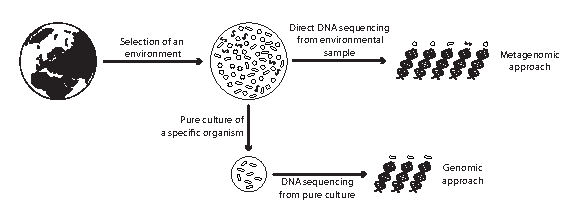
\includegraphics[width=1\textwidth]{./figures/Introduction/metagen_pipeline}
  	\caption{Schematic workflow of a metagenomic and a genomic pipeline. Metagenomics can in principle access 100\% of the genetic material of an environment; whereas traditional cultivation methods and traditional genomics can access to less than 1\%.
  	\label{fig:metapipe}}
\end{figure}

\subsubsection{Who is there: rRNA phylotyping}
As previously said, since many microbes resist being cultured, the usage of culture-independent techniques for identifying and studying microorganisms in their environment has become very popular over the last several decades. These techniques, which have fundamentally changed the fields of microbiology and microbial ecology, have their roots in the analysis of 16S rRNA genes isolated and sequenced directly from the environment, the so-called rRNA phylotyping \cite{pace1997molecular, olsen1986microbial}. This method is based on the huge amount of rRNA gene sequences that have been collected and stored in dedicated databases for the purpose of reconstructing the universal Tree of Life \cite{brown2002universal}. By determining the sequence of an organism’s rRNA genes, it is possible to position it on the appropriate branch of the Tree of Life and infer that its biological characteristics are likely to be similar to those of its closest relatives, the nearest branches on the tree (see~\ref{fig:rnaphylo}).\\
\begin{figure}[!tb]
	\centering
	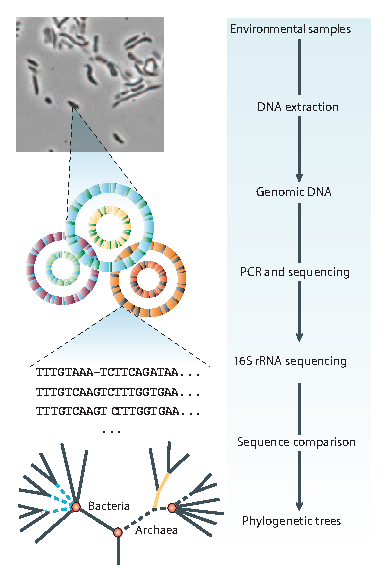
\includegraphics[width=0.5\textwidth]{./figures/Introduction/rna_phylotyping}
  	\caption{Schematic representation of a rRNA phylotype pipeline. In these studies DNA is extracted directly from an environmental sample such as ocean water, soil or a biofilm, and the 16S genes of the community microbes are then amplified from the mixed genomic DNA using PCR. The PCR products are cloned into vectors and sequenced, producing a set of rRNA signatures corresponding to the microbes that were present in the sample. Comparison of these sequences with databases of 16S ribosomal RNA genes allows them to be phylogenetically classified. The frequencies of particular small subunit (SSU) rRNA clone sequences provide a rough preliminary estimate of the community structure, as sequences from dominant community members should be more abundant (from \cite{tringe2005metagenomics}).\label{fig:rnaphylo}}
\end{figure}
An organism does not have to be culturable to determine its phylotype. The polymerase chain reaction (PCR) allows rRNA genes to be isolated and copied directly from environmental samples thanks to its peculiar structure. In particular, the 16S rRNA gene is composed by a succession of highly conserved regions (used for designing PCR primer sequences) and variable ones (used as markers for phylotyping), which makes this gene a perfect target for both PCR amplification and phylotyping. As a consequence, if a sample contains many types of organisms, many different rRNA sequences will be amplified and sequenced, reflecting an high diversity and, likely, an high complexity. Through the classification of the rRNA gene sequence it is possible to answer one of the most controversial question of biology: ``who is there?''. Phylotyping has revolutionized the field of microbiology, and hundreds of environments have been studied with this method \cite{saulnier2011gastrointestinal, lu2008turkey, biddle2008metagenomic, krober2009phylogenetic}. The majority of the 50 major divisions of Bacteria that have been characterized using their rRNA genes do not yet have any cultured representatives. Despite this great amount of data produced, the rRNA phylotyping in itself, should not be considered ``pure'' metagenomics since it focuses on only one gene, not entire genomes. However, this technique is still commonly used as preliminary step in many metagenomics project because it is able to provide a general overview of the microbial diversity of a particular environment with low efforts.\\
Currently, the 16S based approach to the study of microbial communities has some limitations. First, 16S rRNA sequences provide a phylogenetic framework into which community members can be placed, but that framework does not tell us almost anything about the functional capabilities of the individual members or the entire community. In addition, PCR based studies are biased in that not all rRNA genes are amplified equally well with the same primers. In other words, despite the efforts made for designing ``universal'' PCR primers, their sequence will always be based on already existant rRNA sequences so it could never be considered as ``true universal''. Indeed, in several published metagenomics studies, there have been discrepancies between the estimations of microbial diversity obtained with PCR based techniques and those obtained with whole-genome data, although in other studies these estimations were very similar \cite{liles2003census, tyson2004community}. Another limitation is the low resolution power of the current classification algorithms that ranges from the taxonomic level of \textit{Phylum} to that of \textit{Genus}, making this method not suited for high-resolution analyses. The last important limitation of these studies is that rRNA genes occur in multiple copies in many bacteria and archaea, which may lead to over-representation of some species in gene libraries. However, this limitation might be overcome through the use of additional, single-copy phylogenetic markers, such as recA or rpoB, for initial community surveys. Unfortunately, research is still needed for the development of additional markers of community diversity in order to enhance the phylogenetic resolution of microbial communities.\\

\subsubsection{What are they doing: exploring metagenomes}
Organizing genetic information from macroscopic organisms (animals or plants) into phylogenetic trees in order to examine how they are related to one another assumes that all the individuals of a given species have virtually identical genomes. Studies on human genome have revealed that it differs from one another by only 0.1\% allowing different human individuals to be collocated in the same branch of the Tree of Life. On the other hand, the huge amount of microbial genomes has shown that even if culturability ceased to be a problem, diversity will always be a challenge. Indeed, almost all phylotyping surveys of almost all environments have highlighted that a single microbial species can have hundreds of very close but unquestionably nonidentical phylotypes that form a multitude of different clusters instead of a single phylotype. In addition to these small differences in the sequences of the marker genes used in phylotyping, these organisms, in principle members of the same species, differ substantially in the genes that their genomes contain (by up to 30\%) \cite{thompson2005genotypic}. In this perspective the number of genomes that would have to be sequenced in a whole-genome-based metagenomics program would be in the order of thousands or even millions reflecting the high genomic diversity of the bacterial world. As a consequence, one of the biggest challenge faced by microbiologists today may be to understand the biological significance of such phylotypic and genomic variability, and this challenge cannot be completed with a traditional genomic approach.\\
A microbial community can be composed by many different members which differ vastly in their biochemical activities and interactions, not only between species but also within species. The structure of the 16S rRNA gene has allowed phylotyping to give some reliable information about ``Who is there?'' but because of the within-species genomic diversity, we can only guess ``What are they doing''. Such understanding can be achieved only with methods that go beyond the pure-culture and single-whole-genome approaches that have dominated microbial genomics for years. Researchers have to focus directly on the genes in order to characterize environments by the potential activities of the microbial individuals that are there, and the complex patterns of interactions within and between them, which are able to regulate their responses to changes in their environment. In metagenomics, necessity not only is the mother of invention but will be the grandmother of a paradigm shift. Indeed, it has shifted the emphasis from individuals to interactions, from parts to processes, a change that would be highly desirable even if it were not also technologically necessary.\\
As with genomics, many metagenomics projects focused on obtaining enough sequence information to generate almost complete genomes of some or all of a community’s members. Given that environmental samples contain DNA from many species that are present in different abundance and differ from each other in their genome size, the final depth of sequence coverage for each organism at a given level of sequencing will vary. Piecing together all the separately sequenced fragments of a genome is a substantial bioinformatics challenge. In a simple community is possible to obtain enough overlapping fragments of the dominant members to assemble their entire genomes. On the other hand, in a more complex community, even the sequence fragments from the dominant members may be very few precluding the assembly, and species of low abundance might be represented by only a few sequences. However, even if assembling all genomes of a complex community may be a very complex task, these differences in sequence coverage can provide precious informations on relative species abundance. It is important to take differential species representation into account in selecting assembly strategies for metagenomic data to avoid classifying sequences from the most abundant species as repeats and throwing them out of assembly algorithms.\\
Despite the use of some common methods for analysing the genomic information obtained, metagenomics differs from traditional genomic sequencing in many ways. Indeed, metagenomics requires greater attention to sampling procedures, and assessing the diversity of the sample by various means (16S rRNA phylotyping, T-RFLP molecular fingerprinting, Hybridization-based analyses) is necessary to ensure that the sample is representative. Extracting the appropriate quantity of genetic material from the sample is another step that can be very challenging in a metagenomics project. The DNA collected can then either be sequenced (via generation of a library or directly through next-generation sequencing technologies) or assessed for the functions it encodes. Raw sequences can sometimes be assembled into complete genomes of community members, but can also be analysed in other ways (data binning, clustering, comparison with other community). Data storage and computational analyses are critical steps in metagenomics projects and must be integrated throughout the project.\\

\subsubsection*{Organizing metagenomic data}
As said before, working with metagenomic data is not trivial and the development of new tools and methods for analysing metagenomic sequences is becoming mandatory for the correct analysis of the huge amount of data produced every year. Many metagenomic projects aim to obtain large genomic sequences of the representatives of a bacterial community for studying the structure and the functions of that community. Despite the large amount of metagenomic data produced in the last decade there is still the need of a shared metagenomic pipeline like the one used for genomic studies (see~\ref{par:genomics}). This could be due to the high complexity of community data, which are difficult to organize and understand even from the most skilled microbiologists. Currently, a set of bioinformatic tools have been developed in order to cope with all problems related this kind of studies. These tools can be grouped into 4 main categories based on their usage:
\vspace{-5mm}
\begin{itemize}[nosep]
\item Clustering algorithms
\item Binning algorithms
\item Gene prediction algorithms
\item Gene annotation algorithms
\end{itemize}

\paragraph{Clustering algorithms} use an approach to data analysis in which a large dataset is divided into distinct subsets based on some specific measure. In analyzing DNA or protein sequences, clustering is used to identify groups of sequences that share an evolutionary origin (families) but can also identify larger sets, such as genomes (see binning). Genome annotations can be viewed as form of clustering, where individual genes are assigned to well-characterized (or at least previously known) gene families. In metagenomics, direct clustering of DNA sequences is likely to remain a primary annotation method, as most of these sequences will not be easily assigned to any known gene family. In direct clustering, the nucleotide (or predicted protein) sequence itself is the basis of the grouping of sequences.\\

\paragraph{Binning algorithms} are clustering method that uses composition and/or other characteristics of DNA contigs (overlapping individual reads) to divide them into groups (clusters) that belong to specific genomes or groups of genomes. Examples of characteristics that can be used for binning are $GC$ content and codon use. In metagenomic projects in which genome assembly is a goal, this is used as a preliminary step.\\

\paragraph{Gene prediction algorithms} these algorithms are similar to those used in genomic studies. They analyse DNA sequences to predict which encode biological functions, such as coding for proteins, structural and regulatory RNA, and other regulatory elements. Gene prediction is important for determining the functional repertoire of a microbial community and for comparing the capabilities of different communities.\\

\paragraph{Gene annotation algorithms} even these algorithms are similar to their equivalent used in genomic projects. They are able to predict which sequence encode biological functions, such as coding for proteins, structural and regulatory RNA, and other regulatory elements. Gene prediction is important for determining the functional repertoire of a microbial community and for comparing the capabilities of different communities.\\

%%-----------
%% Backmatter
%%-----------
\backmatter
\chaptermark{Bibliography}
\renewcommand{\sectionmark}[1]{\markright{#1}}
\bibliographystyle{unsrt}                           %Use alpha codes for references
\sectionmark{Bibliography}
\addcontentsline{toc}{chapter}{Bibliography}        %Force addition of Bibliography to TOC    
\bibliography{References}